\section{The Quantum Abstract Machine:  Syntax and Semantics} \label{sec:qam}

\begin{figure}[t]
{\small
  \[\begin{array}{llcl} 
      \texttt{Variable} & x,y \\
      \texttt{Message Names} & m &\in& \mathbb{M}\\
    \texttt{Quantum Channel} & c &\in& \Ls\\
      \texttt{Named Quantum Message} & q &::=& m\mid \up{\kappa}\\
      \texttt{Message} & \mathpzc{q} &::=& q \mid \wideparen{q} \mid \circ \\
      \texttt{Channeled Message} & \kappa &::=& \mathpzc{q} \mid c(\kappa) \\
      \texttt{Topped Message} & \eta &::=& \kappa \mid \top \mid c(\eta) \\
    \texttt{Quantum Channel} & c &\in& \Ls\\
    \texttt{Classical Channel} & \wideparen{c} &\in& \Ls\\
    \texttt{Time Stamp} & t &\in& \mathbb{T}\\
\ignore{
    \texttt{Timed Label} & \alpha^t &::=& \qsend{p}{c}{m}^{t}\\
    \texttt{Label} & \iota &::=& c.m \mid p.c.m \mid \alpha^t \mid \emptyset\\
} 


      \texttt{Action} & A & ::= & \downa{c}\,\mid \,\upa{c}\mid \encode{c.\kappa} \mid \decode{c.x} \mid \chan{c.\kappa}\mid \msga{c}{x} \mid \csenda{\wideparen{c}}{\wideparen{m}}\mid\creva{\wideparen{c}}{x} \\[0.2em]

      \texttt{Process} & P,Q & ::= & 0 \mid AP\mid \parp{P}{Q}\mid \comp{P} \\[0.2em]
      \texttt{Top Process} & R & ::= &\pscell{\overline{P}}{\overline{c(\eta)}} \mid P\pscell{\overline{P}}{\overline{c(\eta)}} \\[0.2em]
      \textcolor{red}{\texttt{Configuration First Pattern}} & \textcolor{red}{C} & \textcolor{red}{::=} & \textcolor{red}{\overline{R}}
    \end{array}
  \]
}
\caption{Quantum Abstract Machine Syntax Table}
  \label{fig:q-pi-syntax}
\end{figure}

Here, we first describe a system models single location communication, via the quantum teleportation and GHZ channel building algorithms in \Cref{sec:qamsyntax}, then a system models multiple location communication, via quantum routing in \Cref{sec:qamsyntax1},
and formalize an evaluation framework based on the model in \Cref{sec:qamsemantics1}.

We define QAM system to represent the transitions for any quantum network protocols, which allows programmers to define initial configurations, representing the initial programs and process environment, as well as user-definable transition rules, guiding how configurations are transitioned. A QAM system is a structure $(\Ms,\Ls,\Ts,\overline{\rules})$,
where $\Ms$ is a set of messages;
$\Ls$ is a set of channels;
$\Ts$ is a set of time stamps that forms a linear order ($<$) with $0$ being the minimum;
and $\overline{\rules}$ is a finite set of rules for guiding how configurations are transitioned. 
Any rule has the form $C_1 \xrightarrow{\alpha} C_2$, referring to that we transition configuration $C_1$ to $C_2$ via a label $\alpha$, being either emptily internal ($\emptyset$), a pair $c.m$, a triple $p.c.m$, or a quadruple $(p.c.m)^t$, where $c$ is the channel for communication, $m$ is a possibly quantum message, $p$ is the success rate of the message delivery, and $t$ is the initial time stamp of the message. In QAM, rules are not allowed to associated with side conditions, and we provide special ways of such definitions, explained in \Cref{sec:qamsyntax1}.

The execution in QAM is with respect to a QAM system $(\Ms,\Ls,\Ts,\overline{\rules})$ and an initial configuration $C$ that defines the input program and initial process environment.
If we collect the free metavariables ($\cn{FV}(-)$) appearing in a configuration and rule, 
the initial configuration $C$ is a \textit{ground term} without any metavariables ($\cn{FV}(C)=\emptyset$);
while $\cn{FV}(\alpha) \cup \cn{FV}(C_2)\subseteq \cn{FV}(C_1)$ for every rule $C_1 \xrightarrow{\alpha} C_2$, which is the well-formedness assumption for a QAM system.
We can define the transitions in a QAM system as follows:

\begin{definition}\label{def:labeledsystem}\rm[One QAM Transition Step]
Given a QAM system $\Cs=(\Ms,\Ls,\Ts,\overline{\rules})$ and a ground term initial configuration $C$, a transition step defining for a rule $C_1 \xrightarrow{\alpha} C_2 \in \overline{\rules}$ on $C$ is given as:
\begin{itemize}
\item There is a substitution $\sigma$ mapping every metavariable in $C_1$ to a term, such that $\sigma(C_1)=C$, where we substitute metavariables $x$ in $C_1$ with the mapped terms as $\sigma(x)$.
\item The result label and configuration by applying the rule is $\sigma(\alpha)$ and $\sigma(C_2)$.
\end{itemize}
\end{definition}

\Cref{def:labeledsystem} provides an abstraction of transitions in QAM, where the details configurations and rules are parameterized as some abstract objects.

\subsection{Single Location Communication} \label{sec:qamsyntax}


\begin{figure}[t]
{\footnotesize
$\textcolor{blue}{\text{Message Algebra:}}\\$
\[
\begin{array}{l}
c(\eta) \equiv c.\eta
\quad
c(\circ)\equiv c
\quad
\circ \sqcap \eta \equiv \eta
\quad
\kappa \sqcap \kappa' \equiv \top\;\cn{when}\;\kappa \neq \kappa' \wedge \kappa'\neq \circ
\quad
\wideparen{\kappa}\; \sqcap \up{\kappa} \equiv \kappa
\quad
\wideparen{\kappa} \sqcap \wideparen{\kappa} \equiv \circ
\quad
\eta \sqcap \top = \top
\end{array}
\]

$\textcolor{blue}{\text{Semantics:}}$
  \begin{mathpar}

   \inferrule[Merge]{}
       { \pard{\pscell{P}{\overline{c(\eta)}}}{\pscell{Q}{\overline{c(\eta)}}}
             \longrightarrow \pscell{\pard{P}{Q}}{\overline{c(\eta)}}}
\qquad
   \inferrule[Purge]{c\not\in FV(\overline{P})}
       { \pscell{P}{c(\kappa),\overline{c(\eta)}}
             \longrightarrow \pscell{P}{\overline{c(\eta)}}}
\qquad
   \inferrule[Clean]{}
       {\pscell{\emptyset}{\overline{c(\eta)}} \longrightarrow \emptyset }
\qquad
   \inferrule[ID1]{}
       {\pard{0}{P} \longrightarrow P}

   \inferrule[Cohere]{}
       { \pscell{\pard{\down{c}{P}}{\down{c}{Q}}}{\overline{c(\eta)}}
             \longrightarrow \pscell{\pard{P}{Q}}{c,\overline{c(\eta)}}}
\qquad
   \inferrule[Decohere]{}
       {\pscell{\pard{P}{...}}{\overline{c(\eta)}} \longrightarrow \pard{\pscell{...}{\overline{c(\eta)}}}{\scell{P}} }
\qquad
   \inferrule[ID]{}
       {\pard{\scell{0}}{R} \longrightarrow R}

   \inferrule[Join]{}
       { \pard{\pscell{\pard{\upa{c}{P}}{Q}}{c,\overline{c(\eta)}}}
                    {\pscell{\pard{\upa{c}{P'}}{Q'}}{c,\overline{c(\eta)}}}
             \longrightarrow \pard{\pscell{\pard{Q}{Q'}}{c,\overline{c(\eta)}}}{\pscell{\pard{P}{P'}}{\overline{c(\eta)}}}}
\qquad
  \inferrule[CL]{}
      {\parp{P}{Q} \longrightarrow P}
\qquad
  \inferrule[CR]{}
      {\parp{P}{Q} \longrightarrow Q}

   \inferrule[Encode]{\cn{chan}(\kappa)\not\in \cn{chan}({c(\eta),\overline{c(\eta)}})}
       {\pscell{\pard{\encode{c.\kappa}P}{Q}}{c(\eta),\overline{c(\eta)}} \longrightarrow \pscell{\pard{P}{Q}}{c(\kappa\sqcap\eta),\overline{c(\eta)}} }

   \inferrule[Move]{c\not\in \cn{chan}({\overline{c(\eta)}})}
       { \pscell{\pard{\chan{c.\kappa}P}{Q}}{\overline{c(\eta)}}
             \longrightarrow \pscell{\pard{P}{Q}}{c(\kappa),\overline{c(\eta)}}}

   \inferrule[Back]{}
       { \pscell{\pard{\msga{c}{x}P}{Q}}{c(\kappa),\overline{c(\eta)}}
             \longrightarrow \pscell{\pard{P[c.\kappa/x]}{Q}}{\overline{c(\eta)}}}
\qquad
  \inferrule[Com]{}
      { \pard{\csend{\wideparen{c}}{\wideparen{q}}{R}}{\crev{\wideparen{c}}{x}{R'}}
           \xrightarrow{\wideparen{c}.\wideparen{q}} \pard{R}{R'[\wideparen{q}/x]}}

   \inferrule[DecodeC]{\kappa = \circ \vee \kappa = \wideparen{\kappa}}
       {\pscell{\pard{c.\decode{x}P}{{\decode{c.x}Q}}}{c(\kappa),\overline{c(\eta)}} \xrightarrow{c.\kappa} \pscell{\pard{P[\kappa/x]}{{Q[\kappa/x]}}}{\overline{c(\eta)}} }

   \inferrule[DLock]{}
       {\pscell{\pard{P}{...}}{\wideparen{\kappa}} 
             \longrightarrow P\pscell{{...}}{\wideparen{\kappa}} }

   \inferrule[DDrop]{}
       {P\pscell{{...}}{\wideparen{\kappa}}
             \longrightarrow \pscell{\pard{P}{...}}{\wideparen{\kappa}}  }

   \inferrule[DecodeQ]{\kappa \neq \circ \\ \kappa \neq \wideparen{\kappa}}
       {\pscell{{\pard{\decode{c.x}P}{Q}}}{c(\kappa),\overline{c(\eta)}}
                \xrightarrow{c.\kappa} \pard{\pscell{P[\kappa/x]}{\overline{c(\eta)}}}{\pscell{Q}}{c(\up{\kappa}),\overline{c(\eta)}} }

   \inferrule[DecodeM]{\cn{fresh}\;m}
       {\pscell{{\pard{\decode{c.x}P}{Q}}}{c(\top),\overline{c(\eta)}}
                \xrightarrow{c.m} \pard{\pscell{P[m/x]}{\overline{c(\eta)}}}{\pscell{Q}}{c(\up{m}),\overline{c(\eta)}} }

   \inferrule[MT]{}
       {\comp{P} \longrightarrow \pard{P}{\comp{P}}}
      
   \inferrule[NT]{}
       {\comp{P} \longrightarrow 0}
  \end{mathpar}
}
\caption{Single-party communication syntax and semantics. $\cn{chan}(\eta)$ produces the channel of a message, i.e., if $\eta=c(\eta')$, then $c$ is the channel; if $\eta=m$, then $\top$ is the channel.}
  \label{fig:q-pi-semantics1}
\end{figure}

\begin{figure}[t]
{\hspace*{-1em}
\begin{subfigure}[t]{0.57\textwidth}
{\footnotesize
\[
\begin{array}{l}
\pard{\down{c}{\encode{m}\decode{x}{\csend{\wideparen{c}}{x}{0}}}}{
\down{c}{\crev{\wideparen{c}}{u}{\encode{u}0}}
}
\\[1em]
\begin{array}{ll}
(\rulelab{Self})\;
\longrightarrow
&
\pard{\pscell{\encode{m}\decode{x}{\csend{\wideparen{c}}{x}{0}}}{c}}
{\down{c}{\crev{\wideparen{c}}{u}{\encode{u}0}}}

\\[1em]
(\rulelab{Cohere})\;
\longrightarrow
&
\pscell{\pard{\encode{m}\decode{x}{\csend{\wideparen{c}}{x}{0}}}{\crev{\wideparen{c}}{u}{\encode{u}0}}}{c}
\\[1em]
(\rulelab{Encode})\;
\longrightarrow
&
\pscell{\pard{{\decode{x}{\csend{\wideparen{c}}{x}{0}}}}{\crev{\wideparen{c}}{u}{\encode{u}0}}}{c(m)}
\\[1em]
(\rulelab{DecodeQ})\;
\xrightarrow{c.m}
&
\pard{\csend{\wideparen{c}}{\wideparen{m}}{0}}
{\pscell{{\crev{\wideparen{c}}{u}{\encode{u}0}}}{c(\up{m})}}
\\[1em]
(\rulelab{Move})\;
\longrightarrow
&
\pard{\csend{\wideparen{c}}{\wideparen{m}}{0}}
{{\crev{\wideparen{c}}{u}{\encode{u}0}}\pscell{\emptyset}{c(\up{m})}}
\\[1em]
(\rulelab{Com})\;
\xrightarrow{\wideparen{c}.\wideparen{m}}
&
\pard{0}
{{{\encode{\wideparen{m}}0}}\pscell{\emptyset}{c(\up{m})}}
\\[1em]
(\rulelab{Back})\;
\longrightarrow
&
\pard{0}
{\pscell{{{\encode{\wideparen{m}}0}}}{c(\up{m})}}
\\[1em]
(\rulelab{Encode})\;
\longrightarrow
&
\pard{0}
{\pscell{{{0}}}{c(m)}}
\\[1em]
\longrightarrow...
\end{array}
\end{array}
\]
}
\caption{Quantum Teleportation}
  \label{fig:tele-example}
\end{subfigure}
%
\begin{subfigure}[t]{0.38\textwidth}
{\footnotesize
\[
\begin{array}{l}
\pard{\down{c}{\encode{\wideparen{m}}\decode{x}{0}}}{
\down{c}{\decode{x}{0}}
}
\\[1em]
\begin{array}{ll}
(\rulelab{Self})\;
\longrightarrow
&
\pard{\pscell{\encode{\wideparen{m}}\decode{x}{0}}{c}}{
\down{c}{\decode{x}{0}}
}
\\[1em]
(\rulelab{Cohere})\;
\longrightarrow
&
\pscell{\pard{\encode{\wideparen{m}}\decode{x}{0}}{\decode{x}{0}}}{c}
\\[1em]
(\rulelab{Encode})\;
\longrightarrow
&
\pscell{\pard{\decode{x}{0}}{\decode{x}{0}}}{c(\wideparen{m})}
\\[1em]
(\rulelab{DLock1})\;
\longrightarrow
&
\pscell{\pard{\decode{x}{(0)}}{\decode{x}{0}}}{c(\wideparen{m})}
\\[1em]
(\rulelab{DLock2})\;
\longrightarrow
&
\pscell{\decode{x}{(\pard{0}{0})}}{c(\wideparen{m})}
\\[1em]
(\rulelab{DecodeC})\;
\xrightarrow{c.\wideparen{m}}
&
\pard{{0}}{{0}}
\\[1em]
(\rulelab{ID})\;
\longrightarrow
&
0
\end{array}
\end{array}
\]
}
\caption{Super Dense Coding}
  \label{fig:super-example}
\end{subfigure}
}
\caption{Examples of \Cref{fig:q-pi-semantics1}}
\end{figure}

We first investigate the quantum communication between parties in a single location, which models quantum teleportation and GHZ in \Cref{sec:background}.

The syntax is enlightened by different process algebras, such as CHEM, $\Pi$-calculus, and CSP,
as we instantiate QAM configurations as a multiset of processes $\overline{P}$ representing processes being paralleled,
as the red part in \Cref{fig:q-pi-semantics1}.
Each process performs a sequence of actions, which can be
a channel generation action $\downa{c}$ meaning that a quantum channel is created;
an encoding action $\encode{\mathpzc{q}}$ encodes a message $\mathpzc{q}$, quantum or classical, to a quantum channel;
$\encode{\wideparen{c}(x)}$ is also an encoding action but waiting for a message named $x$ in a classical channel $\wideparen{c}$;
A decoding action $\decode{x}$ decodes the message attached in a quantum channel and names it as $x$;
and a classical sending and receiving actions
$\csenda{\wideparen{c}}{\wideparen{m}}$ and $\creva{\wideparen{c}}{x}$, similar to the ones in $\Pi$-calculus.
One thing worth nothing is that every quantum channel $c$ has a classical counterpart $\wideparen{c}$,
which conveys classical messages to different locations or merges these messages to a quantum message.

A single process can be a unit one $0$; $AP$ finishes action $A$ then continues $P$;
replication process $\comp{P}$ refers to that $P$ can repeatedly happen zero or multiple times
and $\parp{P}{Q}$ is a choice operation.
A membrane of multi-processes $\pscell{\overline{P}}{\wideparen{k}}$ represents the multiple processes $\overline{P}$ are sharing a quantum channel named $\wideparen{k}$.

A quantum channel can be understood as a house.
The simplest format is a pure channel $c$ referring to no message occupies the channel $c(\circ)$ (abbreviated as $c$), so it is ready to receive some messages;
$c(q)$ or $c(\wideparen{q})$ means a quantum or classical message occupies the channel $c$, respectively;
while $c(\top)$ means that $c$ contains an unknown message $\top$.

On the top of \Cref{fig:tele-example}, a multiset of two processes show the quantum teleportation implementation in QAM,
where the left process (Alice) sends a quantum message to the right (Bob).
We first apply rule \rulelab{Self} in \Cref{fig:q-pi-semantics1}
to allow Alice herself showing the willingness of creating a quantum channel membrane named $c$,
while the \rulelab{Cohere} rule application joins Bob to the quantum channel by moving Bob to the membrane.
The \rulelab{Self} and \rulelab{Decohere} applications reflect the quantum channel establishment step, as \coqe{bel1000} in \Cref{fig:background-circuit-examplea}.
At this point, it is possible that Bob can lose the quantum channel through the \rulelab{Decohere} rule application nondeterministically.
If that happens, Bob cannot gain back his channel,
referring to the fact that once a party's quantum channel is lost, its qubit resource is also lost.
Rule \rulelab{Clean} removes the empty membrane from a system.

We then apply rule \rulelab{Encode} to push the quantum message $m$ to the channel $c$.
Giving a existing quantum channel $c(\kappa)$ and a new coming message $\mathpzc{q}$,
rule \rulelab{Encode} utilizes function $\sqcap$
to compute the meet of $\mathpzc{q}$ and $\kappa$, as the result of the message pushing.
We design the message and the $\sqcap$ function based on the real-world observations of quantum network communications,
which only have limited kinds of messages. First, there is an initial unit message $\circ$ representing a quantum message being just created without encoding any information, such as a series of $\ket{0}$ qubits.
Second, if we encode a message $\mathpzc{q}$, quantum or classical, with a pure channel that has message $\circ$, the state results in $c(\mathpzc{q})$,
but if we push the same message twice, the behavior erases the message and the state becomes $c(\circ)$.
Third, a general quantum message $m$ is usually transmitted and analyzed through an algorithm that utilize quantum teleportation as a subroutine to convey the message, which means that it can be viewed as a division of two parts: a classical message $\wideparen{m}$ and a quantum remain $\up{m}$, and the two parts can be merged back through the encoding operation back to message $m$.
This behavior is captured by the equation rule $\wideparen{q}\; \sqcap \up{q} \equiv q$ in \Cref{fig:q-pi-semantics1},
where we encode a classical message $\wideparen{q}$ with an existing quantum channel $c(\up{q})$ that has the quantum remain $\up{q}$;
in such case, the encoding results in $c(q)$.
Fourth, the other cases are rarely used in the current quantum protocols, and we view them as some unknown state captured by $\top$ and we develop the decoding rule \rulelab{DecodeM} to capture such behavior. In such case, there will be a new fresh message generated in the system.

We then apply rule \rulelab{DecodeQ} to destory the channel $c(m)$, so that Alice holds a classical portion of the message $\wideparen{m}$, while Bob holds the quantum remain $\up{m}$. The above two rule applications model the \coqe{alice} application in \Cref{fig:background-circuit-examplea}, to destroy a quantum message $m$.

The rest rule applications in \Cref{fig:tele-example}, especially \rulelab{Com} and \rulelab{Encode}, model the \coqe{bob} application in  \Cref{fig:background-circuit-examplea}, allowing Bob to recover the message $m$.
Rule \rulelab{Com} delivers the classical message $\wideparen{m}$ that Alice holds to Bob, which is a traditional $\Pi$-calculus message communication rule, while rule \rulelab{Encode} pushes $\wideparen{m}$ to the channel $c(\up{m})$, so the final state of the channel becomes $c(m)$, holding the message $m$.

\Cref{fig:super-example} provides an example transitions for modeling the super dense coding algorithm,
the key idea is that a classical message $\wideparen{m}$ can be attached to an initial quantum channel $c$, and the rule \rulelab{DecodeC} application mimics the measurement step in the algorithm to produce the classical message $\wideparen{m}$ out of the quantum channel.
In QAM, we utilize the decoding action to measure a quantum channel and produce different results.
In fact, the circuit implementations of the decoding operations for channels containing quantum message $c(m)$ and classical message $c(\wideparen{m})$ are different, but the functionalities are the same, which is why we have different rules (\rulelab{DecodeQ} and \rulelab{DecodeC}) for them.

Rules \rulelab{CL} and \rulelab{CR} in \Cref{fig:q-pi-semantics1} are the semantics for choice operation that nondeterministically choose a process as continuation, while rules \rulelab{MT} and \rulelab{NT} are the semantics for the replication process.
These four rules are inherent from $\Pi$-calculus.

\subsection{Distinct Location Communication} \label{sec:qamsyntax1}

\begin{figure}[t]
{\small
$\textcolor{blue}{\text{Syntax:}}\\$
  \[\begin{array}{llcl} 
      \texttt{Channel Package} & \wideparen{\kappa} & ::= & c(\kappa) \\[0.2em]
      \texttt{Action} & A & ::= & \downa{c}\,\mid \encode{\mathpzc{q}} \mid \encode{\wideparen{c}(x)} \mid \decode{x} \mid \csenda{\wideparen{c}}{\wideparen{m}}\mid\creva{\wideparen{c}}{x} \\[0.2em]

      \texttt{Process} & P,Q & ::= & 0 \mid AP\mid \parp{P}{Q}\mid \comp{P}
              \mid \pscell{\overline{P}}{\wideparen{\kappa}?}_{\textcolor{red}{\overline{c}}} \\[0.2em]
      \textcolor{red}{\texttt{Membrane Process Abbr.}} & \textcolor{red}{P^{\wideparen{\kappa}?}_{\overline{c}}} &
                 \textcolor{red}{::=} & \textcolor{red}{\pscell{\overline{P}}{\wideparen{\kappa}?}_{\overline{c}}}\\[0.2em]
    \textcolor{red}{\texttt{Relation Pairs}} & \textcolor{red}{S} 
        & \textcolor{red}{::=} & \textcolor{red}{\overline{c_1 \to c_2}} \\[0.2em]
      \textcolor{red}{\texttt{Configuration First Pattern}} & \textcolor{red}{C} & \textcolor{red}{::=} & \textcolor{red}{\overline{P^{\wideparen{\kappa}?}_{\overline{c}}}}
    \end{array}
  \]

$\textcolor{blue}{\text{Semantics:}}\\$
  \begin{mathpar}
   \inferrule[Self]{}
       {\scell{\down{c}{P}}_{c_1} \longrightarrow \pscell{P}{c}_{c_1}}

   \inferrule[Cohere1]{|\overline{c}|\le 1\\c_1\to c_2 \in S}
       { \pard{\pscell{...}{c}_{\overline{c},c_1}}{P^c_{c_2}} \xrightarrow{c_1\to c_2}
           \pscell{\pard{...}{P}}{c}_{\overline{c},c_1,c_2}}

   \inferrule[Decohere]{}
       {\pscell{\pard{P}{...}}{\wideparen{\kappa}}_{c_1,\overline{c}} \longrightarrow 
           \pard{\pscell{...}{\wideparen{\kappa}}_{\overline{c}}}{\scell{P}_{c_1}} }

   \inferrule[Comm]{}
       { \pscell{P,Q}{\wideparen{\kappa}}_{c_1,c_2} \longrightarrow \pscell{Q,P}{\wideparen{\kappa}}_{c_2,c_1}}

   \inferrule[Swap]{}
       { \pscell{\pard{\pard{P}{\down{c}P'}}{Q}}{c}_{c_1,c_2,c_3}
           \longrightarrow  \pard{\pscell{\pard{P}{Q}}{c}_{c_1,c_3}}{\scell{P'}_{c_2}} }

   \inferrule[Clean]{}
       {\pscell{\emptyset}{\wideparen{\kappa}}_{\overline{c}} \longrightarrow \emptyset }

   \inferrule[Encode]{}
       {\pscell{\pard{\encode{\mathpzc{q}}P}{...}}{c(\kappa)}_{\overline{c}} \longrightarrow \pscell{\pard{P}{...}}{c(\mathpzc{q}\,\sqcap\kappa)}_{\overline{c}} }

   \inferrule[Move]{}
       {\pscell{\pard{P}{...}}{\wideparen{\kappa}}_{\overline{c}} 
             \longrightarrow P\pscell{{...}}{\wideparen{\kappa}}_{\overline{c}} }

   \inferrule[Back]{}
       {P\pscell{{...}}{\wideparen{\kappa}}_{\overline{c}}
             \longrightarrow \pscell{\pard{P}{...}}{\wideparen{\kappa}}_{\overline{c}}  }

  \inferrule[QCom]{}
      { \pard{\csend{\wideparen{c}}{\wideparen{q}}{P}}{\encode{\wideparen{c}(x)}{Q}}
           \xrightarrow{\wideparen{c}.\kappa} \pard{P}{\encode{\wideparen{q}}Q}}

  \inferrule[Com]{}
      { \pard{\csend{\wideparen{c}}{\wideparen{q}}{P}}{\crev{\wideparen{c}}{x}{Q}}
           \xrightarrow{\wideparen{c}.\wideparen{q}} \pard{P}{Q[\wideparen{q}/x]}}

   \inferrule[Decode01]{}
       {\pscell{\pard{\decode{x}P}{Q}}{c}_{c_1,c_2} \xrightarrow{c.\circ} {\pard{\scell{P[\circ/x]}_{c_1}}{\scell{Q}_{c_2}}} }

   \inferrule[DecodeC1]{}
       {\pscell{\pard{\decode{x}P}{\decode{x}Q}}{c(\wideparen{q})}_{c_1,c_2} \xrightarrow{c.\wideparen{q}}
              \pard{\scell{P[\wideparen{q}/x]}_{c_1}}{\scell{Q[\wideparen{q}/x]}_{c_2}} }

   \inferrule[DecodeQ1]{}
       {\pscell{{\pard{\decode{x}P}{Q}}}{c(q)}_{c_1,c_2}
                \xrightarrow{c.q} {\pard{\scell{P[\overline{q}/x]}_{c_1}}{\pscell{Q}}{c(\up{q})}_{c_2}} }

   \inferrule[DecodeM1]{\cn{fresh}\;m}
       {\pscell{{\pard{\decode{x}P}{Q}}}{c(\top)}_{c_1,c_2}
                \xrightarrow{c.m} \pard{\scell{P[\overline{m}/x]}_{c_1}}{\pscell{Q}{c(\up{m})}_{c_2}} }

   \inferrule[ID]{}
       {\pard{\scell{0}_c}{P} \longrightarrow P}

  \inferrule[CL]{}
      {\parp{P}{Q} \longrightarrow P}

  \inferrule[CR]{}
      {\parp{P}{Q} \longrightarrow Q}

   \inferrule[MT]{}
       {\comp{P} \longrightarrow \pard{P}{\comp{P}}}
      
   \inferrule[NT]{}
       {\comp{P} \longrightarrow 0}
  \end{mathpar}
}
\caption{Distinct location communication syntax and semantics.}
  \label{fig:q-pi-semantics2}
\end{figure}

\ignore{
\begin{figure}[t]

{\small
$\textcolor{blue}{\text{Additional Syntax:}}\\$
  \[\begin{array}{llcl} 
      \texttt{Communication Location Flag} & \beta & ::= & \emptyset \mid c \mid c \rightarrow c\\[0.2em]
      \texttt{Process Cell} & \varphi & ::= & \pcell{\overline{P}}{n}{c}\\[0.2em]
      \textcolor{red}{\texttt{Configuration Second Pattern}} & \textcolor{red}{C} & \textcolor{red}{::=} & 
\textcolor{red}{\overline{\varphi}}
    \end{array}
  \]

$\textcolor{blue}{\text{Semantics:}}\\$
  \begin{mathpar}
\mprset{flushleft}
   \inferrule[GC]{}
       {\pcell{\pard{\alpha^t.P}{...}}{\cn{S}\;i}{c_1}\pcell{ ...}{\cn{S}\;j}{c_2}
        \qcell{\emptyset}{\cn{comm}}
        \longrightarrow \pcell{\pard{P}{...}}{i}{c_1}\pcell{\pard{\alpha^t.0}{...}}{j}{c_2}}
  
  \inferrule[PC]{\overline{P}\xrightarrow{\alpha^t} \overline{Q} }
      { \pcell{\overline{P}}{n}{c}
           \longrightarrow
         \pcell{\overline{Q}}{n}{c}}

  \end{mathpar}
}
\caption{\liyi{Alternative:} Inter-destination communication syntax and semantics. $\beta$ can be omitted when being $\emptyset$. $\alpha^t$ is an action such that $\alpha$ has the form $p.c.m$. $\qsend{p}{c}{m}^t\equiv \qsend{p}{c}{m}^t.0$. $\cn{T}$/$\cn{F}$: true or false values.}
  \label{fig:q-pi-semanticsal2}
\end{figure}
}

\begin{figure}[t]
{\footnotesize
\[
\begin{array}{l}
\begin{array}{l}
Cat\triangleq\down{c}{\encode{m}\decode{x}{\csend{\wideparen{c}}{x}{0}}}
\qquad
Dan\triangleq\down{c}{\crev{\wideparen{c}}{u}{\encode{u}0}}
\qquad
r_1\triangleq \parp{\down{c}r_1}{0}
\end{array}\\
\begin{array}{lll}
&
\pard{\pard{\qcellb{Cat}{\cn{Cat}}}
{\qcellb{Dan}{\cn{Dan}}}}
{\qcellb{r_1}{r_1}}
&
\\[0.5em]
\longrightarrow
&
\pard{\pard{\pscell{\encode{m}\decode{x}{\csend{\wideparen{c}}{x}{0}}}{c}_{\cn{Cat}}}
{\qcellb{r_1}{r_1}}}
{\qcellb{Dan}{\cn{Dan}}}
&
(\rulelab{Self})
\\[0.5em]
\longrightarrow
&
\pard{\pard{\pscell{\encode{m}\decode{x}{\csend{\wideparen{c}}{x}{0}}}{c}_{\cn{Cat}}}
{\qcellb{\down{c}r_1}{r_1}}}
{\qcellb{Dan}{\cn{Dan}}}
&
(\rulelab{CL})
\\[0.5em]
\longrightarrow
&
\pard{\pard{\pscell{\encode{m}\decode{x}{\csend{\wideparen{c}}{x}{0}}}{c}_{\cn{Cat}}}
{\pscell{r_1}{c}_{r_1}}}
{\qcellb{Dan}{\cn{Dan}}}
&
(\rulelab{Self})
\\[0.5em]
\xrightarrow{\cn{Cat}\to r_1}
&
\pard{\pscell{\pard{\encode{m}\decode{x}{\csend{\wideparen{c}}{x}{0}}}{r_1}}{c}_{\cn{Cat},r_1}}
{\qcellb{Dan}{\cn{Dan}}}
&
(\rulelab{Cohere1})
\\[0.5em]
\longrightarrow
&
\pard{\pscell{\pard{\encode{m}\decode{x}{\csend{\wideparen{c}}{x}{0}}}{r_1}}{c}_{\cn{Cat},r_1}}
{\pscell{\crev{\wideparen{c}}{u}{\encode{u}0}}{c}_{\cn{Dan}}}
&
(\rulelab{Self})
\\[0.5em]
\xrightarrow{r_1\to \cn{Dan}}
&
\pscell{\pard{\pard{\encode{m}\decode{x}{\csend{\wideparen{c}}{x}{0}}}{r_1}}
   {\crev{\wideparen{c}}{u}{\encode{u}0}}}{c}_{\cn{Cat},r_1,\cn{Dan}}
&
(\rulelab{Cohere1})
\\[0.5em]
\longrightarrow
&
\pscell{\pard{\pard{\encode{m}\decode{x}{\csend{\wideparen{c}}{x}{0}}}{\down{c}r_1}}
   {\crev{\wideparen{c}}{u}{\encode{u}0}}}{c}_{\cn{Cat},r_1,\cn{Dan}}
&
(\rulelab{CL})
\\[0.5em]
\longrightarrow
&
\pard{\pscell{\pard{\encode{m}\decode{x}{\csend{\wideparen{c}}{x}{0}}}
   {\crev{\wideparen{c}}{u}{\encode{u}0}}}{c}_{\cn{Cat},\cn{Dan}}}
{\scell{r_1}_{r_1}}
&
(\rulelab{Swap})
\\[0.5em]
\longrightarrow
&
\pard{\pscell{\pard{\decode{x}{\csend{\wideparen{c}}{x}{0}}}
   {\crev{\wideparen{c}}{u}{\encode{u}0}}}{c(m)}_{\cn{Cat},\cn{Dan}}}
{\scell{r_1}_{r_1}}
&
(\rulelab{Encode})
\\[0.5em]
\xrightarrow{c.m}
&
\pard{\pard{\scell{{\csend{\wideparen{c}}{\overline{m}}{0}}}_{\cn{Cat}}}
     {\pscell{\crev{\wideparen{c}}{u}{\encode{u}0}}{c(\up{m})}_{\cn{Dan}}}}
  {\scell{r_1}_{r_1}}
&
(\rulelab{DecodeQ1})
\\[0.5em]
\longrightarrow
&
\pard{\pard{\csend{\wideparen{c}}{\overline{m}}{0}\scell{\emptyset}_{\cn{Cat}}}
     {\crev{\wideparen{c}}{u}{\encode{u}0}\pscell{\emptyset}{c(\up{m})}_{\cn{Dan}}}}
  {\scell{r_1}_{r_1}}
&
(\text{two}\;\rulelab{Move})
\\[0.5em]
\xrightarrow{\wideparen{c}.\wideparen{m}}
&
\pard{\pard{0\scell{\emptyset}_{\cn{Cat}}}
     {{\encode{\overline{m}}0}\pscell{\emptyset}{c(\up{m})}_{\cn{Dan}}}}
  {\scell{r_1}_{r_1}}
&
(\rulelab{Com})
\\[0.5em]
\longrightarrow
&
\pard{\pard{\scell{0}_{\cn{Cat}}}
     {\pscell{{\encode{\overline{m}}0}}{c(\up{m})}_{\cn{Dan}}}}
  {\scell{r_1}_{r_1}}
&
(\text{two}\;\rulelab{Back})
\\[0.5em]
\longrightarrow
&
\pard{\pard{\scell{0}_{\cn{Cat}}}
     {\pscell{{0}}{c(m)}_{\cn{Dan}}}}
  {\scell{r_1}_{r_1}}
&
(\rulelab{Encode})
\\[0.5em]
\longrightarrow...
\end{array}
\end{array}
\]
}
\caption{Example transitions based on the model in \Cref{fig:q-pi-semantics2}.}
  \label{fig:q-pi-example}
\end{figure}

Most network communication is performed in distinct locations,
where the channel establishment based on the GHZ algorithm become impractical, when connecting parties residing on more than $3$ locations. As we mentioned in \Cref{sec:background}, a typical quantum routing algorithm relies on the swap concept to build a long distance quantum channel. Here, we upgraded the QAM syntax and semantics in \Cref{fig:q-pi-semantics1} to the system in \Cref{fig:q-pi-semantics2}, by removing GHZ channel building rules and implementing quantum swaps.

We restrict the syntax in \Cref{fig:q-pi-semantics2} based on the system in \Cref{fig:q-pi-semantics1}.
We require every single location process to be surrounded by a membrane structure with a location name $c$, representing a process happening in a location $c$.
On the top level, we have a memtiset of membranes representing communications happening in distinct locations.
Membrane can be abbreviated as $P^{\wideparen{\kappa}?}_{\overline{c}}$, meaning that a process can happen in several locations labeled by the location list $\overline{c}$, and $\wideparen{\kappa}$ is a possible channel associated with the membrane.
Inside each membrane, we can have an ordered list of process, whose cardinality is less than $3$.
The process list in a membrane and the location list associated with the membrane are one-to-one corresponded.
For example, if we have the membrane
$\scell{P,P',Q}_{c_1,c_2,c_3}$,
$c_1$, $c_2$, and $c_3$ are the locations holding the process $P$, $P'$, and $Q$, respectively.
In this system, each evaluation is associated with a relation set $S$, containing the location connectivity.
The other processes and actions are similar to the ones appearing in \Cref{fig:q-pi-semantics1}.

The semantics in \Cref{fig:q-pi-semantics2} are mostly similar to the one in \Cref{fig:q-pi-semantics1}, except that we associate location information with membranes. For all those rules that only differ from the ones in \Cref{fig:q-pi-semantics1} with the membrane structure and location information, we keep the rule names to be the same.

We now explain some semantic rules through an example in \Cref{fig:q-pi-example},
which shows a multiset of three processes that sends a quantum message from \cn{Cat} to \cn{Dan} via a router $r_1$,
with the three process definitions on the top. $r_1$ is a recursive process definition. In these transition steps, we omit the function call steps for $Cat$, $r_1$, and $Dan$ in each membranes.
The first three rule applications (two \rulelab{Self} and one \rulelab{CL}) establish the willingness of communications between membranes \cn{Cat} and $r_1$.
We then apply rule \rulelab{Conhere1}, which models the Bell pair establishment in \Cref{sec:background},
that connects \cn{Cat} and $r_1$ in the same membrane, meaning that they are now sharing the same channel $c$.
During the process, the membrane's location list is now $\cn{Cat},r_1$ and an explicit label $\cn{Cat} to r_1$ is attached to the transition.

After another \rulelab{Self} application, we can then apply \rulelab{Cohere1} again to move \cn{Dan} to the $\cn{Cat},r_1$ membrane,
so the membrane becomes a three-party one, with the location list $\cn{Cat},r_1,\cn{Dan}$.
Even though \cn{Cat} and \cn{Dan} are in the same membrane but they cannot communicate with each other because all rules in \Cref{fig:q-pi-semantics2} are applied on processes across different membranes or between adjacent membranes, but \cn{Cat} and \cn{Dan} are separated by $r_1$. 
To remove $r_1$ from the membrane, we apply rule \rulelab{Swap} to move $r_1$ outside the membrane by losing an additional quantum channel $\down{c}$ in $r_1$.
Then, \cn{Cat} and \cn{Dan} are the only two parties in the membrane $\cn{Cat},\cn{Dan}$, so that we can apply similar encoding and decoding rules as in \Cref{fig:tele-example}.
One thing worth noting is that the consecutive \rulelab{Cohere1} and \rulelab{Swap} application exactly model the swapping procedure in \Cref{sec:background}; that is, by losing two qubit resources, one in \rulelab{Cohere1} application and the other in \rulelab{Swap} application, we first entangle \cn{Dan} and $r_1$ and then swap out $r_1$ so that $\cn{Cat}$ and $\cn{Dan}$ are directly connected.


\ignore{

\begin{definition}\label{def:stuck}\rm[Terminated and Stuck Configurations]
A configuration $C$ is a terminated state if no rule is possible to apply to $C$ and:
\begin{itemize}
\item For all process cell in $C$, its content is a unit process $0$.
\item $\alpha$ and $\beta$ in $\pcell{\alpha}{\beta}{\cn{comm}}$ are $\emptyset$ and $b$ in $\qcell{b}{\cn{pred}}$ is \cn{F}.
\end{itemize}
$C$ is stuck if no rule is possible to apply to it and the above conditions are not satisfied.
\end{definition}

As an example of the QAM syntax, the above configuration defines the initial program state for sending a message $c.m$ from $\cn{Cat}$ to $\cn{Dan}$ via the router $r_1$, as part of the communication in \Cref{fig:q-pi-example}. Initially, the relation cell stores the connectivity between \cn{Cat}, \cn{Dan}, and $r_1$, with the success rates. 
The global time is initialized as $0$ in the \cn{gt} cell, and the predicate cell has a fixed value $\texttt{false}$.
The message ($\qsend{1}{c}{m}$) sent from \cn{Cat} has an initial probability value $1$.
Node $r_0$ acts as a intermediate router, so it only contains the unit process $0$, and \cn{Dan} is waiting on receiving a message ($\qrev{c}{x}.0$). 

\begin{figure}[t]
{\small
  \begin{mathpar}
\mprset{flushleft}
   \inferrule[GC]{}
       {\Cellb{\qsend{p}{c}{m}^t}{i}{c_1}\Cella{P}{j}{c_2} \qcell{\{(c_1,c_2,p')\}\cup R}{\cn{rel}}\qcell{t'}{\cn{gt}}
        \qcell{\emptyset}{\cn{comm}}\pcell{b}{\_}{\cn{pred}}
       \\\\\qquad\qquad \longrightarrow \Cellb{}{i-}{c_1}\Cella{\qsend{p*p'}{c}{m}^{t}\texttt{|}P}{j-}{c_2}
              \qcell{\{(c_1,c_2,p')\}\cup R}{\cn{rel}}\qcell{t'}{\cn{gt}}
               \qcell{(c_1,c_2,\qsend{p}{c}{m}^t)}{\cn{comm}}\pcell{b}{t'}{\cn{pred}}}

\ignore{
   \inferrule[GenQubit]{}
       {\Cella{P}{n,t'}{a}\qcell{t}{\cn{gt}}\longrightarrow \Cella{P}{n+,t}{a}\qcell{t}{\cn{gt}}}\;\;\texttt{when}\;t \texttt{|} \beta\wedge t' < t
}

   \inferrule[CT]{}
       {\Cellb{\parl{\qsend{p}{c}{m}.P}{Q}}{i}{c_1}\qcell{t}{\cn{gt}} 
         \longrightarrow \Cellb{\pard{\qsend{p}{c}{m}.P}{Q}}{i}{c_1}\qcell{t}{\cn{gt}}}

   \inferrule[MT]{}
       {\comp{P} \longrightarrow \parl{P}{\comp{P}}}
      
   \inferrule[NT]{}
       {\comp{P} \longrightarrow 0}

  \inferrule[PC]{}
      { \Cellb{\qsend{p}{c}{m}^t\texttt{|} \qrev{c}{x}.P}{n}{c}\qcell{t'}{\cn{gt}}\qcell{\emptyset}{\cn{comm}}\pcell{b}{\_}{\cn{pred}}
           \longrightarrow
         \Cellb{P[m/x]}{n}{c}\qcell{t'}{\cn{gt}}\qcell{\qsend{p}{c}{m}^t}{\cn{comm}}\pcell{b}{t'}{\cn{pred}}}
                  

  \inferrule[Com]{}
      { \qcell{t'}{\cn{gt}}\qcell{\qsend{p}{c}{m}^t}{\cn{comm}}\pcell{\cn{true}}{t'}{\cn{pred}}
           \xrightarrow{p.c.m}  
         \qcell{t'+}{\cn{gt}}\qcell{\emptyset}{\cn{comm}}\pcell{\cn{false}}{t'}{\cn{pred}} } 

  \inferrule[FC]{}
      { \qcell{t}{\cn{gt}}\qcell{(c_1,c_2,A)}{\cn{comm}}\pcell{\cn{true}}{t}{\cn{pred}}
           \longrightarrow
         \qcell{t+}{\cn{gt}}\qcell{\emptyset}{\cn{comm}}\pcell{\cn{false}}{t}{\cn{pred}} } 

  \end{mathpar}
}
\caption{Quantum Pi Semantics. $\beta$, $\mu$, and $\nu$ are globally defined for the qubit generation period, the message threshold probability, and message sending finished threshold. $\Cella{P}{n}{a}$ refers to that the $t$ in $\Cella{P}{n,t}{a}$ is omitted in the rule.}
  \label{fig:q-pi-semantics}
\end{figure}
}

\ignore{
\begin{figure}[t]
{\small
{\hspace*{-2em}
\begin{tikzpicture}[align=center,node distance=1.5cm and -1cm, thick] 
\node (1) {S$\langle\{(a,r_1,0.5), (a,r_2,0.5)\}\cup$R$\rangle$}; 
\node (2) [below left= of 1] {$\Cella{0}{9}{a}$ $\Cella{\qsend{0.5}{c}{m}|0}{9}{r_1}$... $\langle\{(r_1,r_4)\}\cup$R$\rangle$}; 
\node (3) [below right= of 1] {\text{\ \ \ \ \ \ }$\Cella{0}{9}{a}$ $\Cella{\qsend{0.5}{c}{m}|0}{9}{r_2}$..., $\ccell{\{(r_2,r_3)\}\cup\text{R}}$}; 
\node (4) [below of=2] {$\Cella{0}{8}{r_1}$ $\Cella{\qsend{0.25}{c}{m}|0}{9}{r_4}$... $\langle\{(r_4,b)\}\cup$R$\rangle$};
\node (5) [below of=3] {\text{\ \ \ \ \ \ }$\Cella{0}{8}{r_2}$ $\Cella{\qsend{0.25}{c}{m}|0}{9}{r_3}$..., $\ccell{\{(r_3,r_4)\}\cup\text{R}}$};
\node (6) [below of=4] {$\Cella{0}{8}{r_4}$ $\Cella{\qsend{0.125}{c}{m}|\qrev{c}{x}.0}{9}{b}$... $\ccell{\text{R}}$};
\node (7) [below of=5] {\text{\ \ \ \ \ \ \ \ \;}$\Cella{0}{8}{r_3}$ $\Cella{\qsend{0.125}{c}{m}|0}{9}{r_4}$..., $\ccell{\{(r_4,b)\}\cup\text{R}}$};
\node (8) [below of=6] {$\Cella{0}{9}{b}$... $\ccell{\text{R}}$};
\node (9) [below of=7] {\text{\ \ \ \ \ \ \ \ }$\Cella{0}{8}{r_4}$ $\Cella{\qsend{0.0625}{c}{m}|\qrev{c}{x}.0}{9}{b}$..., $\ccell{\text{R}}$};
\node (10) [below of=9] {\text{\ \ \ \ \ \ }$\Cella{0}{n}{b}$... $\ccell{\text{R}}$};
\draw[->] (1) -- node[midway, above left] {} (2); 
\draw[->] (1) -- node[midway, above right] {} (3); 
\draw[->] (2) -- node[midway, right] {} (4); 
\draw[->] (4) -- node[midway, right] {} (6);
\draw[->] (6) -- node[midway, right] {$0.125.c.m$} (8); 
\draw[->] (3) -- node[midway, right] {} (5); 
\draw[->] (5) -- node[midway, right] {} (7); 
\draw[->] (7) -- node[midway, right] {} (9);
\draw[->] (9) -- node[midway, right] {$0.0625.c.m$}  (10); 
\end{tikzpicture} 
}
}
\caption{Quantum Machine Transitions for \Cref{fig:q-pi-example}}
  \label{fig:q-pi-example1}
\end{figure} 
}


\subsection{Adding Connectivity and Time Stamps} \label{sec:qamsemantics1}

\begin{figure}[t]
{\small
$\textcolor{blue}{\text{Extended Syntax:}}\\$
  \[\begin{array}{llcl} 
      \texttt{Time Predicate Function} & f & \in & \Ts \times \Ts \to \cn{bool} \\[0.2em]
      \texttt{Relation} & R & ::= & \overline{(c,c,p)}  \\[0.2em]
      \textcolor{red}{\texttt{Configuration Third Pattern}} & \textcolor{red}{C} & \textcolor{red}{::=} & 
\textcolor{red}{\overline{\varphi}\pcell{\alpha}{\beta}{\cn{comm}}
  \qcell{\cn{bool}}{\cn{pred}}\qcell{R}{\cn{rel}}\qcell{t}{\cn{gt}} }
    \end{array}
  \]

$\textcolor{blue}{\text{Semantics:}}\\$
  \begin{mathpar}
\mprset{flushleft}
   \inferrule[GC1]{}
       {\pcell{\pard{\qsend{p}{c}{m}^t.P}{...}}{\cn{S}\;i}{c_1}\pcell{ ...}{\cn{S}\;j}{c_2}
        \qcell{\emptyset}{\cn{comm}}
        \qcell{\pard{(c_1,c_2,p')}{...}}{\cn{rel}}
        \\\\ \qquad \longrightarrow \pcell{\pard{P}{...}}{i}{c_1}\pcell{\pard{\qsend{p'\cn{*}p'}{c}{m}^t}{...}}{j}{c_2}
               \pcell{(p \cn{*} p'.c.m)^t}{c_1\rightarrow c_2}{\cn{comm}}
        \qcell{\pard{(c_1,c_2,p')}{...}}{\cn{rel}}}

   \inferrule[CT]{}
       {\pcell{\pard{\qsend{p}{c}{m}.P}{...}}{i}{c_1}\qcell{t}{\cn{gt}} \longrightarrow 
             \pcell{\pard{\qsend{p}{c}{m}^t.P}{...}}{i}{c_1}\qcell{t}{\cn{gt}}}

\textcolor{blue}{
  \inferrule[PC]{\overline{P}\xrightarrow{\alpha^t} \overline{Q} }
      { \pcell{\overline{P}}{n}{c}\qcell{\emptyset}{\cn{comm}}
           \longrightarrow
         \pcell{\overline{Q}}{n}{c}\pcell{\alpha^t}{c}{\cn{comm}}}
}
               
   \inferrule[Grant1]{}
       {\qcell{\cn{F}}{\cn{pred}}\pcell{\alpha}{c_1\rightarrow c_2}{\cn{comm}}
             \longrightarrow \qcell{\cn{T}}{\cn{pred}}\pcell{\alpha}{c_1\rightarrow c_2}{\cn{comm}}}
  
   \inferrule[Grant2]{}
       {\pcell{\alpha^t}{c}{\cn{comm}}\qcell{\cn{F}}{\cn{pred}}\qcell{t'}{\cn{gt}} 
     \longrightarrow \pcell{\alpha^t}{c}{\cn{comm}}\qcell{f(t,t')}{\cn{pred}}\qcell{t'}{\cn{gt}}}

  \inferrule[FC1]{}
      { \pcell{\alpha}{c_1\rightarrow c_2}{\cn{comm}}\qcell{\cn{T}}{\cn{pred}}\qcell{t}{\cn{gt}}
           \longrightarrow \qcell{\emptyset}{\cn{comm}}\qcell{\cn{F}}{\cn{pred}}\qcell{t\cn{+}}{\cn{gt}} } 
 
  \inferrule[AC1]{}
      { \pcell{\alpha^t}{c}{\cn{comm}}\qcell{\cn{T}}{\cn{pred}}\qcell{t}{\cn{gt}}
           \xrightarrow{\alpha}  \qcell{\emptyset}{\cn{comm}}\qcell{\cn{F}}{\cn{pred}}\qcell{t\cn{+}}{\cn{gt}} } 

  \end{mathpar}
}
\caption{Extended inter-destination communication syntax and semantics. $\beta$ can be omitted when being $\emptyset$. $\alpha^t$ is an action such that $\alpha$ has the form $p.c.m$. $\qsend{p}{c}{m}^t\equiv \qsend{p}{c}{m}^t.0$.}
  \label{fig:q-pi-semantics3}
\end{figure}

\begin{figure}[t]
{\small
$\textcolor{blue}{\text{Extended Syntax:}}\\$
  \[\begin{array}{llcl} 
      \texttt{Time Predicate Function} & f & \in & \Ts \times \Ts \to \cn{bool} \\[0.2em]
      \texttt{Relation} & R & ::= & \overline{(c,c,p)}  \\[0.2em]
      \textcolor{red}{\texttt{Configuration Third Pattern}} & \textcolor{red}{C} & \textcolor{red}{::=} & 
\textcolor{red}{\overline{\varphi}\qcell{\beta}{\cn{comm}}\qcell{R}{\cn{rel}}\qcell{t}{\cn{gt}} }
    \end{array}
  \]

$\textcolor{blue}{\text{Semantics:}}\\$
  \begin{mathpar}
\mprset{flushleft}
   \inferrule[GC1]{}
       {\pcell{\pard{\alpha^t.P}{...}}{\cn{S}\;i}{c_1}\pcell{ Q}{\cn{S}\;j}{c_2}\qcell{\emptyset}{\cn{comm}}
    \longrightarrow \pcell{\pard{P}{...}}{i}{c_1}\pcell{\parl{\alpha^t.0}{Q}}{j}{c_2}\qcell{c_1\to c_2}{\cn{comm}}
     }

   \inferrule[Cohere1]{}
       {\pcell{\parl{\alpha(p)^t.P}{Q}}{i}{c_2}
        \qcell{\pard{(c_1,c_2,p')}{...}}{\cn{rel}}
     \qcell{c_1\to c_2}{\cn{comm}}\qcell{t'}{\cn{gt}}
    \\\qquad\longrightarrow 
       \pcell{\pard{\alpha(p\cn*{p'})^t.P}{Q}}{i}{c_2}
        \qcell{\pard{(c_1,c_2,p')}{...}}{\cn{rel}}
     \qcell{\emptyset}{\cn{comm}}\qcell{t'\cn{+}}{\cn{gt}}
     }
     \quad{\cn{when}\;\;f(t,t')}

   \inferrule[Break1]{}
       {\pcell{\parl{\alpha(p)^t.P}{Q}}{i}{c_2}
     \qcell{c_1\to c_2}{\cn{comm}}\qcell{t'}{\cn{gt}}
    \longrightarrow 
       \pcell{Q}{i}{c_2}
     \qcell{\emptyset}{\cn{comm}}\qcell{t'\cn{+}}{\cn{gt}}
     }
     \quad{\cn{when}\;\;\neg f(t,t')}

   \inferrule[CT]{}
       {\pcell{\pard{\alpha.P}{...}}{i}{c_1}\qcell{t}{\cn{gt}} \longrightarrow 
             \pcell{\pard{\alpha^t.P}{...}}{i}{c_1}\qcell{t}{\cn{gt}}}

\textcolor{blue}{
  \inferrule[PC]{\overline{P}\xrightarrow{\alpha^t} \overline{Q} }
      { \pcell{\overline{P}}{n}{c}\qcell{t'}{\cn{gt}}
           \xrightarrow{\alpha^t}
         \pcell{\overline{Q}}{n}{c}\qcell{t'\cn{+}}{\cn{gt}}}
}

  \end{mathpar}
}
\caption{\liyi{Alternative} Extended inter-destination communication syntax and semantics. $\beta$ can be omitted when being $\emptyset$. $\alpha^t$ is an action such that $\alpha$ has the form $p.c.m$. $\qsend{p}{c}{m}^t\equiv \qsend{p}{c}{m}^t.0$.}
  \label{fig:q-pi-semanticsal3}
\end{figure}


\begin{figure}[h]
\begin{center}
 \begin{subfigure}[b]{0.4\textwidth}
     \centering
    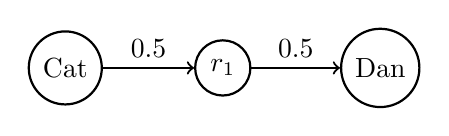
\begin{tikzpicture}[node distance={2cm}, thick, main/.style = {draw, circle}] 
    \node[main] (1) {\cn{Cat}}; 
    \node[main] (2) [right of=1] {$r_1$};
    \node[main] (3) [right of=2] {\cn{Dan}};
    \draw[->] (1) -- node[midway, above] {0.5} (2); 
    \draw[->] (2) -- node[midway, above] {0.5} (3);  
    \end{tikzpicture}
    \caption{Cat too Dan}
    \label{fig:y equals x}
\end{subfigure}
\hfill
 \begin{subfigure}[b]{0.4\textwidth}
     \centering
    \begin{tikzpicture}[node distance={2cm}, thick, main/.style = {draw, circle}] 
    \node[main] (5) [below of=2] {\cn{Ann}};
    \node[main] (6) [right of=5] {\cn{Bob}};
    \draw[->] (5) -- node[midway, below] {0.5} (6);
    % \draw[dashed] (2) -- (5);
    \end{tikzpicture}
    \caption{Cat to Dan \& Ann to Bob}
    \label{fig:y equals x}
\end{subfigure}

\end{center}
\caption{Example Path Connectivity }
  \label{fig:examplepath}
\end{figure}
As in \Cref{sec:qamsyntax1}, QAM permits a quantum protocol semantics through the manipulation of configurations and rules describing the communicating, granting, and cleaning steps for framing quantum network communications.
Here, we extend the configuration and rules in \Cref{fig:q-pi-semantics2} to define two important properties appearing in almost all quantum network protocols: connectivity and time.
The former refers to that quantum messages are always transmitted based on a connectivity graph, i.e., two cells can communicate if they have an edge in the graph and each edge has a certain success rate of message transmission. One example connectivity is in \Cref{fig:examplepath}.
The latter means that quantum messages are time-sensitive and are required to deliver in a short lifetime; otherwise, the messages are decohered and lost.

To define the two properties, we extend the configuration with the \cn{gt} and \cn{rel} cells in \Cref{fig:q-pi-semantics3},
which respectively contain a global clock time $t$ and a multiset of relation triples $R$ whose element is a triple of source and target cell locations and the success rate to transmit a message from the source to the target.
A user defined validity check function $f$ is used to determine if a message spends too much time in its transmission.
\Cref{fig:q-pi-semantics3} shows the semantic rule definitions for the two properties. Rule \rulelab{PC} is marked blue because it keeps the same as the case in \Cref{fig:q-pi-semantics2}, while the other rules require some modifications, explained below.
 
\noindent\textbf{Defining connectivity.}
Definition the property requires the update of rule \rulelab{GC} to \rulelab{GC1} in \Cref{fig:q-pi-semantics3}
by including the extra \cn{rel} cell.
In each message ($\qsend{p}{c}{m}^t$) transmission, we pattern match the source $c_1$ and target $c_1$ locations in the \cn{rel} cell as $(c_1,c_2,p')$. After the message is transmitted, we reduce its success rate as $p\cn{*}p'$, referring to that the message transmission results in a success rate reduction.

\noindent\textbf{Defining time.}
Definition this property is essentially two procedures.
First, a global time clock is introduced in the cell \cn{gt}.
In the upgraded rules (\rulelab{FC1} and \rulelab{AC1}) for cleaning steps, we include the \cn{gt} cell and increments the clock ($t\cn{+}$). We also include a new rule \rulelab{CT} to generate time stamp label for a message, so that we can mark the sending time of the message correctly. Second, we need to define a new granting rule by applying the validity check function $f$ to verify if a message's delivery is past due. To do so, we split the granting rule (\rulelab{Grant} in \Cref{fig:q-pi-semantics2}) into two rules.
For the case of message transmission (flag $c_1 \rightarrow c_2$ in \cn{comm}), it keeps the same;
otherwise, we apply function $f$ on a pair of time stamps, indicating the starting time of the message ($t$) and the final delivery time ($t'$), respectively. Function $f$ is user-defined. One example definition could be a lambda abstraction $\lambda\,(t,t')\,.\,t'-t<m$, where $m$ is a threshold time period for a message guaranteeing to deliver.

\begin{figure}[t]
{\footnotesize
\[\hspace*{-1em}
\begin{array}{lll}
&
\pcellb{\qsend{1}{c}{m}.0}{10}{\cn{Cat}}
\pcellb{0}{10}{r_1}
\pcellb{\qrev{c}{x}.0}{10}{\cn{Dan}} 
\qcellb{\emptyset}{\cn{comm}}
\qcellb{\texttt{F}}{\cn{pred}}
\qcellb{R}{\cn{rel}}
\qcellb{0}{\cn{gt}}
&
\\[0.3em]
\longrightarrow
&
\pcellb{\qsend{1}{c}{m}^0.0}{10}{\cn{Cat}}
\pcellb{0}{10}{r_1}
\pcellb{\qrev{c}{x}.0}{10}{\cn{Dan}} 
\qcellb{\emptyset}{\cn{comm}}
\qcellb{\texttt{F}}{\cn{pred}}
\qcellb{R}{\cn{rel}}
\qcellb{0}{\cn{gt}}
&
(\rulelab{CT})
\\[0.3em]
\longrightarrow
&
\pcellb{0}{9}{\cn{Cat}}
\pcellb{\qsend{0.5}{c}{m}^0.0}{9}{r_1}
\pcellb{\qrev{c}{x}.0}{10}{\cn{Dan}} 
\pcellb{(1.c.m)^0}{\cn{Cat}\rightarrow r_1}{\cn{comm}}
\qcellb{\texttt{F}}{\cn{pred}}
\qcellb{R}{\cn{rel}}
\qcellb{0}{\cn{gt}}
&
(\rulelab{GC1})
\\[0.3em]
\longrightarrow
&
\pcellb{0}{9}{\cn{Cat}}
\pcellb{\qsend{0.5}{c}{m}^0.0}{9}{r_1}
\pcellb{\qrev{c}{x}.0}{10}{\cn{Dan}} 
\pcellb{(1.c.m)^0}{\cn{Cat}\rightarrow r_1}{\cn{comm}}
\qcellb{\texttt{T}}{\cn{pred}}
\qcellb{R}{\cn{rel}}
\qcellb{0}{\cn{gt}}
&
(\rulelab{Grant1})
\\[0.3em]
\longrightarrow
&
\pcellb{0}{9}{\cn{Cat}}
\pcellb{\qsend{0.5}{c}{m}^0.0}{9}{r_1}
\pcellb{\qrev{c}{x}.0}{10}{\cn{Dan}} 
\qcellb{\emptyset}{\cn{comm}}
\qcellb{\texttt{F}}{\cn{pred}}
\qcellb{R}{\cn{rel}}
\qcellb{1}{\cn{gt}}
&
(\rulelab{FC1})
\\[0.3em]
\longrightarrow ...
\\[0.3em]
\longrightarrow
&
\pcellb{0}{9}{\cn{Cat}}
\pcellb{0}{8}{r_1}
\pcellb{\pard{\qsend{0.25}{c}{m}^0.0}{\qrev{c}{x}.0}}{9}{\cn{Dan}} 
\qcellb{\emptyset}{\cn{comm}}
\qcellb{\texttt{F}}{\cn{pred}}
\qcellb{R}{\cn{rel}}
\qcellb{2}{\cn{gt}}
&
\\[0.3em]
\longrightarrow
&
\pcellb{0}{9}{\cn{Cat}}
\pcellb{0}{8}{r_1}
\pcellb{0}{9}{\cn{Dan}} 
\pcellb{(0.25.c.m)^0}{\cn{Dan}}{\cn{comm}}
\qcellb{\texttt{F}}{\cn{pred}}
\qcellb{R}{\cn{rel}}
\qcellb{2}{\cn{gt}}
&
(\rulelab{Com},\rulelab{PC1})
\\[0.3em]
\longrightarrow
&
\pcellb{0}{9}{\cn{Cat}}
\pcellb{0}{8}{r_1}
\pcellb{0}{9}{\cn{Dan}} 
\pcellb{(0.25.c.m)^0}{\cn{Dan}}{\cn{comm}}
\qcellb{f(0,2)}{\cn{pred}}
\qcellb{R}{\cn{rel}}
\qcellb{2}{\cn{gt}}
&
(\rulelab{Grant2})
\\[0.3em]
\xrightarrow{0.25.c.m}&
\pcellb{0}{9}{\cn{Cat}}
\pcellb{0}{8}{r_1}
\pcellb{0}{9}{\cn{Dan}} 
\qcellb{\emptyset}{\cn{comm}}
\qcellb{\texttt{F}}{\cn{pred}}
\qcellb{R}{\cn{rel}}
\qcellb{3}{\cn{gt}}
&
(\rulelab{AC1})
\end{array}
\]
}
{\footnotesize
\begin{center}
$R\triangleq\{(\cn{Cat},r_1,0.5), (r_1,\cn{Dan},0.5)\}$
\qquad
$f=\lambda\,(t,t')\,.\,t'-t<5$
\end{center}
}
\caption{Example transitions based on the model in \Cref{fig:q-pi-semantics3}.}
  \label{fig:q-pi-example1}
\end{figure}


\Cref{fig:q-pi-example1} shows an example evaluation of the initial configuration on the top,
which is an instantiation of metavariables in configuration pattern in \Cref{fig:q-pi-semantics3}.
We first apply rule \rulelab{CT} to generate time stamp $0$ for the sending process action $\qsend{0.25}{c}{m}$.
We then apply rule \rulelab{GC1} and the two consecutive rules to transmit the action to cell $r_1$.
We can perform rule \rulelab{GC1} because the triple $(\cn{Cat},r_1,0.5)$ is in $R$.
During the steps, a piece of qubit resouce is consumed in both \cn{Cat} and $r_1$ cells, the action's success rate is reduced to $0.5$, and the global clock is updated to $1$.
After another round of message transmission steps, the action is conveyed to cell \cn{Dan}.
We then use rule \rulelab{PC}, with rule \rulelab{Com}, to deliver the action.
with the rule applications \rulelab{Grant2} and \rulelab{AC1} to grant and clean the delivery.
The delivery is granted, because the validity check results in $f(0,2)=2-0<5=\cn{T}$.

On the other hand, if users set the validity check function to be $\lambda\,(t,t')\,.\,t'-t<2$,
the validity check here results in $f(0,2)=2-0<2=\cn{F}$, which means that the evaluation is stuck at the \rulelab{Grant2} step.







